\documentclass[a4paper,12pt]{report}
\usepackage{graphicx}
\title{Report\\``MTSK-GAME''}

\author{Pietro Olivi\\
Leonardo Tassinari\\
Lorenzo Dalmonte\\
Alessio Paoloni}
\date{\today}


\begin{document}

\maketitle

\tableofcontents

\chapter{Analysis}
The software commissioned by the professors of the Object Oriented Pro\-gramming course aims to create an application designed to enhance psycho-motor skills through a gaming experience based on multitasking.\\
The term \textit{Multitasking} refers to the ability of a person or a product to do more than one thing at a time.

\section{Requirements}
\subsection*{Functional}
\begin{itemize}
	\item Upon starting, the software will display a simple minigame.\\
	A minigame is a potentially-never-ending challenge that requires simple actions from the player in order to keep the game going.
	After a short amount of time a new minigame will appear and so on until all four minigames are shown.
	\item The player's goal is to survive as long as possible. After failing a minigame the application will display the final result, 
  therefore the software has to keep track of how long the player has lasted in the match in order to calculate the score.
\end{itemize}

\subsection*{Non functional}
\begin{itemize}
	\item The application shall sustain high framerate (around 120 fps) in all the sections of the gameplay, even on older hardware\footnote{e.g. Intel Core i3 (fourth generation), 4Gb of RAM.}.
	\item It shall be possible to easily develop and swap the minigames among the ones that best fit the training purposes of the user on top of those already provided. 
\end{itemize}



\section{Domain analysis}

MTSK-Game must exhibit some \textit{minigames}, the ones supplied by us are:
\begin{itemize} 
	\item \textit{WhacAMole}: where the goal is to crush all the moles that emerge from the dug holes, before they re-enter them.
	\item \textit{DodgeATriangle}: in which the player has to slide a \textit{rectangle} up and down switching lanes, aiming to avoid hitting moving \textit{triangles}.
	\item \textit{CatchTheSquare}: where the user should collect \textit{squares} running over them with a \textit{circle} before they disappear.
	\item \textit{FlappyBirdAlike}: where the user needs to control a \textit{cursor} leading it to fit between \textit{obstacles} that will come towards it.
\end{itemize}
For the game to end, and the \textit{score} to appear, it'll be sufficient losing in only one of the currently displayed mingames.


\begin{figure}[ht]
	\centering{}
	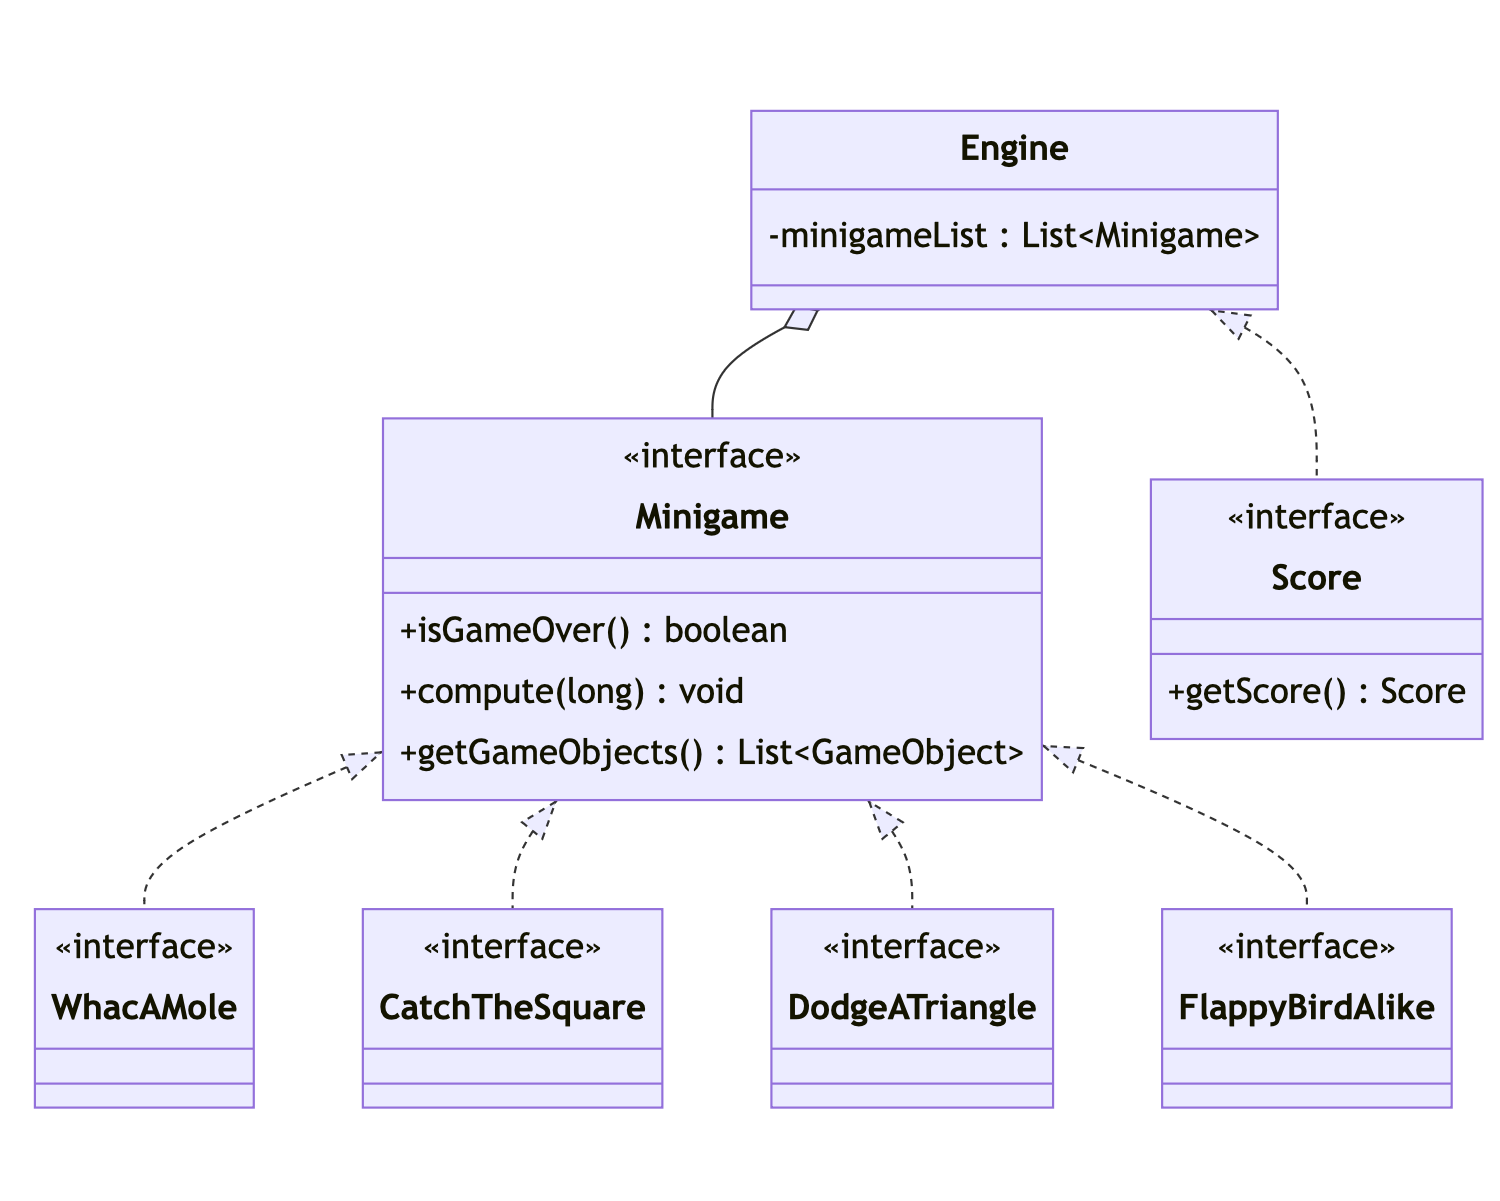
\includegraphics[width=\textwidth]{domain.png}
	\caption{UML diagram of the domain analysis}
\end{figure}

\chapter{Design}

\section{Architecture}
The project is built on the "model-view-controller" architecture: the \textbf{Engine} class represents the controller, hence the entry point of the program.
Inside the controller we create an instance of the \textbf{View}, SwingView in our case, which takes care of intercepting the user's input, then forwarded to the Engine,
and deals with the graphical representation of each minigame. The engine also contains a list of minigames, each of which provides its own implementation of the \textbf{Minigame} interface, that forms the logic.
Once the input has been received, the Engine is responsible for communicating it to each minigame: these in turn will update the state of all the GameObjects they contain, i.e. every single entity in the various playing fields.
The Model part and the View part have an indirect link: the Drawings class. In fact, each GameObject is characterized by a series of specifications (Drawings), contained in the AspectModel, which the View is able to interpret 
to draw the object in the GUI.

\section{Detailed design}
Each minigame is composed of \textbf{GameObject}s: those items use a component pattern, thanks to which we get 
a full separation of concerns based on domains (allow a single entity to span multiple domains each other \footnote{From GPP, CH 14}).
\pagebreak
\begin{itemize}
	\item \textit{PhysicsModel}: Interface that deals with the physical state of a Game Object,
	moving it according to its speed, considering the environment in which it is located (edges of the field) 
	and the other objects it interacts with (collision with obstacles).
	\item \textit{AspectModel}: It is the interface that orders the updating of the graphics of the single 
	object to the View, specifying which of the instructions already contained in SwingView need to be used.
	\item \textit{InputModel}: Interface related to a single GameObject that reads the input stored in the 
	engine and applies it, if the object recognizes it as its own command, changing its specifications (e.g. coordinates, speed).
\end{itemize}

\begin{figure}[ht]
	\centering{}
	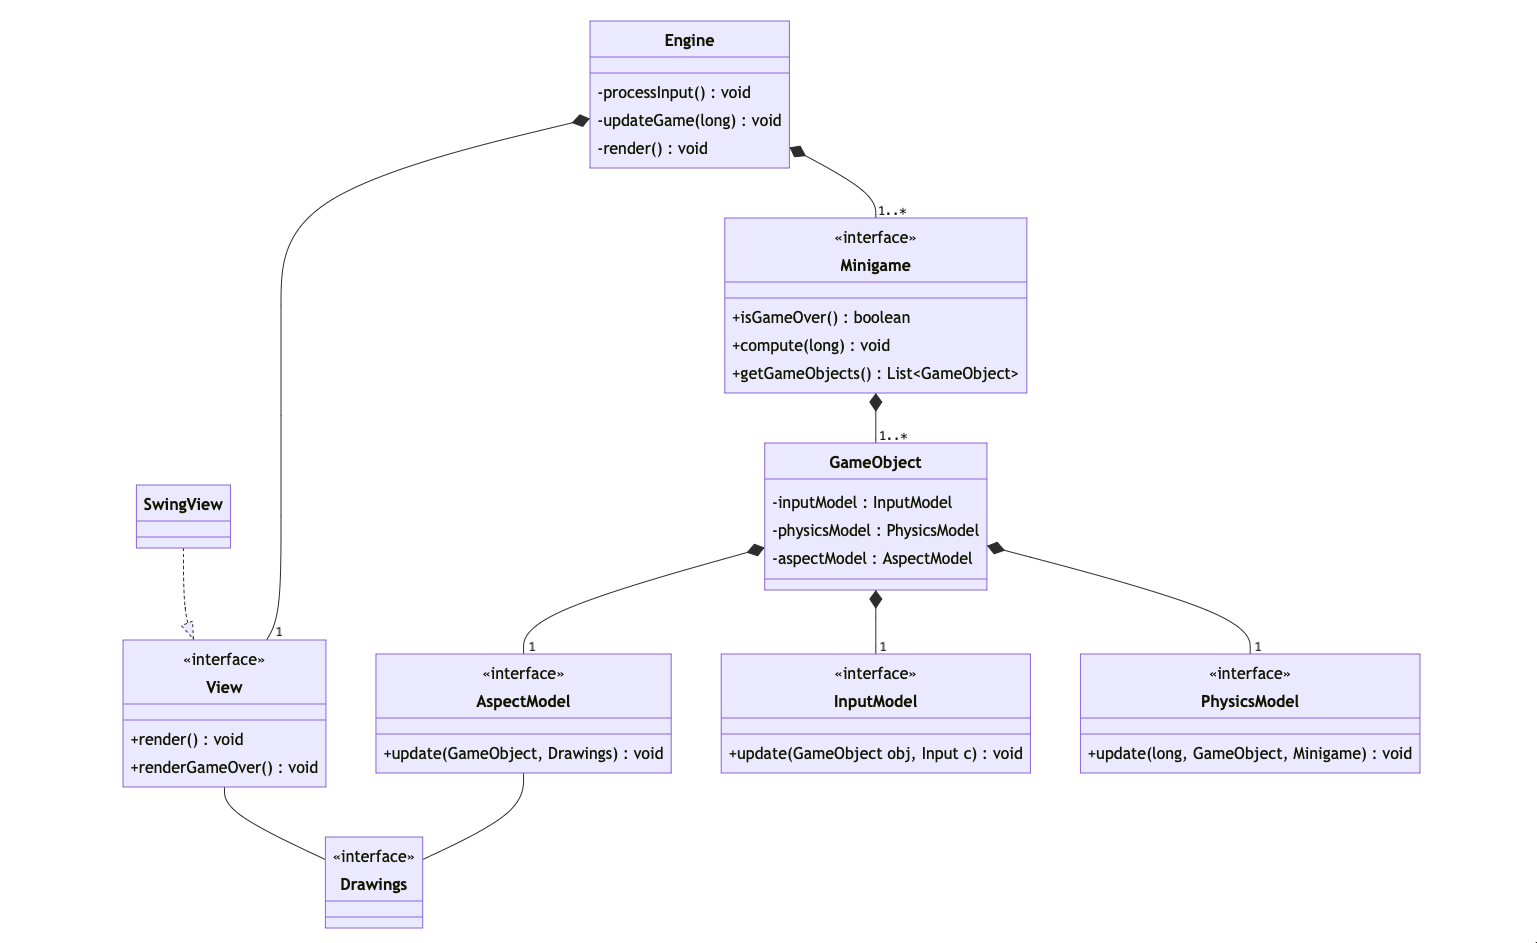
\includegraphics[width=\textwidth]{architecture.png}
	\caption{UML diagram of the architecture}
\end{figure}

\end{document}
